% ============================================================
%  MIVA-KNIGHT Pipeline C: RAVDESS Standalone Audio Emotion Training
%  Complete Technical Documentation
%  Student: Kayode (Oluwakayode) Soyinka | IT 581 Capstone
% ============================================================
\documentclass[12pt,a4paper]{article}

%% ── Encoding & fonts ─────────────────────────────────────────
\usepackage[utf8]{inputenc}
\usepackage[T1]{fontenc}

%% ── Geometry ─────────────────────────────────────────────────
\usepackage[margin=2.4cm,top=2.8cm,bottom=2.8cm]{geometry}

%% ── Mathematics ──────────────────────────────────────────────
\usepackage{amsmath,amssymb,amsthm,mathtools}
\usepackage{bm}

%% ── Algorithms ───────────────────────────────────────────────
\usepackage{algorithm}
\usepackage{algpseudocode}
\algnewcommand\algorithmicinput{\textbf{Input:}}
\algnewcommand\algorithmicoutput{\textbf{Output:}}
\algnewcommand\INPUT{\item[\algorithmicinput]}
\algnewcommand\OUTPUT{\item[\algorithmicoutput]}
\renewcommand{\algorithmiccomment}[1]{\hfill$\triangleright$ \textit{#1}}

%% ── TikZ ─────────────────────────────────────────────────────
\usepackage{tikz}
\usetikzlibrary{
  shapes.geometric, shapes.misc,
  arrows.meta, arrows,
  positioning, calc, fit,
  backgrounds,
  decorations.pathreplacing,
  patterns, matrix
}
\usepackage{pgfplots}
\pgfplotsset{compat=1.18}

%% ── Tables & Boxes ───────────────────────────────────────────
\usepackage{booktabs,array,tabularx,multirow,longtable}
\usepackage{tcolorbox}
\tcbuselibrary{skins,breakable,theorems}
\usepackage{xcolor}

%% ── Formatting ───────────────────────────────────────────────
\usepackage{enumitem}
\usepackage{titlesec}
\usepackage{fancyhdr}
\usepackage{graphicx}
\usepackage{float}
\usepackage{hyperref}
\hypersetup{colorlinks=true,linkcolor=NavyBlue,urlcolor=NavyBlue}
\usepackage{cancel}   % strikethrough

%% ── Colour palette ───────────────────────────────────────────
\definecolor{NavyBlue}{RGB}{20,60,120}
\definecolor{CoralRed}{RGB}{210,80,70}
\definecolor{SlateGray}{RGB}{80,100,120}
\definecolor{MintGreen}{RGB}{60,160,110}
\definecolor{Amber}{RGB}{200,140,30}
\definecolor{Lavender}{RGB}{120,90,170}
\definecolor{DeepTeal}{RGB}{20,100,100}
% Box fills (GCN palette adapted)
\definecolor{BoxBlue}{RGB}{210,225,245}
\definecolor{BoxRed}{RGB}{245,215,215}
\definecolor{BoxOrange}{RGB}{255,232,205}
\definecolor{BoxGray}{RGB}{228,228,228}
\definecolor{BoxGreen}{RGB}{200,235,210}
\definecolor{BoxPurple}{RGB}{228,215,242}
\definecolor{BoxDark}{RGB}{45,45,60}
\definecolor{DarkContainer}{RGB}{195,210,232}

%% ── Theorem environments ─────────────────────────────────────
\theoremstyle{definition}
\newtheorem{definition}{Definition}[section]
\newtheorem{axiom}{Axiom}[section]

\theoremstyle{plain}
\newtheorem{theorem}{Theorem}[section]
\newtheorem{lemma}{Lemma}[section]
\newtheorem{corollary}{Corollary}[section]
\newtheorem{proposition}{Proposition}[section]

\theoremstyle{remark}
\newtheorem{remark}{Remark}[section]

%% ── tcolorbox styles ─────────────────────────────────────────
\tcbset{
  layman/.style={
    enhanced,breakable,
    colback=BoxOrange!55,colframe=Amber!80,
    fonttitle=\bfseries\small,
    title={Simple Explanation},
    left=5pt,right=5pt,top=4pt,bottom=4pt,
    before skip=5pt,after skip=5pt
  },
  notebox/.style={
    enhanced,breakable,
    colback=BoxGreen!55,colframe=MintGreen!80,
    fonttitle=\bfseries\small,
    left=5pt,right=5pt,top=4pt,bottom=4pt,
    before skip=4pt,after skip=4pt
  }
}

%% ── Page style ───────────────────────────────────────────────
\pagestyle{fancy}
\fancyhf{}
\fancyhead[L]{\small\textcolor{NavyBlue}{MIVA-KNIGHT Pipeline C --- RAVDESS Audio Emotion Training}}
\fancyhead[R]{\small\textcolor{NavyBlue}{IT 581 --- Kayode Soyinka}}
\fancyfoot[C]{\thepage}
\renewcommand{\headrulewidth}{0.4pt}

%% ── Section formatting ───────────────────────────────────────
\titleformat{\section}[block]
  {\large\bfseries\color{NavyBlue}}{\thesection}{1em}{}[\titlerule]
\titleformat{\subsection}[block]
  {\normalsize\bfseries\color{SlateGray}}{\thesubsection}{1em}{}
\titleformat{\subsubsection}[runin]
  {\normalsize\bfseries\color{DeepTeal}}{\thesubsubsection}{0.5em}{\ }[.]

%% ── TikZ node styles (GCN-inspired) ─────────────────────────
\tikzset{
  basebox/.style={rectangle,rounded corners=4pt,draw=black!55,
    align=center,font=\small},
  inputbox/.style={basebox,fill=BoxDark,text=white,
    minimum width=2.6cm,minimum height=1.4cm},
  procbox/.style={basebox,fill=BoxBlue,thick,
    minimum width=3.0cm,minimum height=1.2cm},
  trainbox/.style={basebox,fill=BoxRed,
    minimum width=3.0cm,minimum height=1.2cm},
  lossbox/.style={basebox,fill=BoxOrange,thick,
    minimum width=3.2cm,minimum height=1.2cm},
  outbox/.style={basebox,fill=BoxGreen,
    minimum width=3.0cm,minimum height=1.2cm},
  infbox/.style={basebox,fill=BoxGray,
    minimum width=3.0cm,minimum height=1.2cm},
  centbox/.style={basebox,fill=BoxPurple,
    minimum width=3.0cm,minimum height=1.2cm},
  arrow/.style={->,>=Stealth,thick,color=black!70},
  thickarrow/.style={->,>=Stealth,very thick,color=black},
  redarrow/.style={->,>=Stealth,thick,color=CoralRed!80},
  greenarrow/.style={->,>=Stealth,thick,color=MintGreen!80},
  dasharrow/.style={->,>=Stealth,thick,dashed,color=black!50},
  purplearrow/.style={->,>=Stealth,thick,color=Lavender!80}
}

% ============================================================
\begin{document}
% ============================================================

%% ── Title page ───────────────────────────────────────────────
\begin{titlepage}
\centering
\vspace*{1.8cm}
{\Huge\bfseries\color{NavyBlue} MIVA-KNIGHT}\\[0.5cm]
{\Large\color{SlateGray} Pipeline C: RAVDESS Standalone Audio Emotion Training}\\[0.3cm]
{\large\color{SlateGray} Supervisor-Mandated Replan $\mid$ Audio-Only Supervised Contrastive Learning}\\[1.4cm]

\begin{tcolorbox}[notebox,width=0.88\textwidth,
  title={Complete Technical Documentation --- Pipeline C}]
\centering
\textbf{Algorithms, Theorems, Lemmas, Flowchart \& Dual-Language Explanations}\\[0.4cm]
This document provides the complete mathematical derivation, formal
theorem and lemma statements, pseudocode algorithms, TikZ pipeline
flowchart, and dual-language (technical + layman) explanations for
every component of the MIVA-KNIGHT Pipeline~C implementation.
\end{tcolorbox}

\vspace{1.2cm}
\begin{tabular}{@{}ll}
\textbf{Student:}  & Kayode (Oluwakayode) Soyinka \\[3pt]
\textbf{Course:}   & IT 581 --- Capstone Project \\[3pt]
\textbf{Pipeline:} & C --- RAVDESS Standalone Audio Emotion \\[3pt]
\textbf{Dataset:}  & RAVDESS (1,440 clips, 8 emotions, 24 actors) \\[3pt]
\textbf{Loss:}     & Supervised Contrastive (SupCon, Khosla et al.\ 2020) \\[3pt]
\textbf{Hardware:} & Google Colab T4 GPU (15\,GB VRAM) \\[3pt]
\textbf{Runtime:}  & $\approx$27 min on T4 GPU ($\approx$60 min on CPU) \\
\end{tabular}

\vspace{2cm}
\tableofcontents
\end{titlepage}

% ============================================================
\section{System Overview and Design Axioms}
% ============================================================

\subsection{What Pipeline C Solves}

Pipeline~C addresses two critical failures in the original Month~2 implementation:

\begin{tcolorbox}[notebox,title={Two Bugs Fixed by Pipeline C}]
\textbf{Bug 1 --- Contaminated joint training:} RAVDESS audio was trained jointly with
COCO images under one InfoNCE loss.  COCO and RAVDESS share no genuine cross-modal
ground truth.  Synthetic captions (``A person expressing happy emotion'') were pushed
apart as negatives, corrupting the 512-d shared embedding space.
Result: Month 3 SupCon reduced audio emotion accuracy from 5/8 to 2/8.

\textbf{Bug 2 --- Wrong Wav2Vec dimension:} The original cache stored RAVDESS
embeddings at 512d.  Wav2Vec 2.0 base outputs 768d hidden states.  This made
AudioProjection a near-identity $512\to512$ map with almost no learning capacity.
\end{tcolorbox}

\begin{axiom}[Standalone Modality Training]
Audio emotion representations should be learned from audio labels alone,
without cross-modal entanglement from unrelated datasets.  The only valid
supervisory signal for RAVDESS is the emotion label embedded in each filename.
\end{axiom}

\begin{axiom}[Correct Feature Dimensionality]
Wav2Vec 2.0 base outputs $768$-dimensional hidden states.  All pipeline components
must be initialised with this correct dimension; using a different value produces
a near-identity projection with negligible learning capacity.
\end{axiom}

\begin{axiom}[Unit Hypersphere Embeddings]
All modality projections in MIVA-KNIGHT output L2-normalised unit vectors on
$\mathbb{S}^{511} \subset \mathbb{R}^{512}$, so that cosine similarity equals
the standard inner product and is consistent across all retrieval and contrastive
components.
\end{axiom}

\subsection{Component Summary}

\begin{center}
\renewcommand{\arraystretch}{1.2}
\begin{tabular}{@{}llrr@{}}
\toprule
\textbf{Component} & \textbf{Status} & \textbf{Parameters} & \textbf{Receives Gradients?} \\
\midrule
Wav2Vec 2.0 (backbone) & Frozen & 94\,M & No \\
AudioProjection (head) & Trainable & $\approx$987\,K & Yes \\
SupCon loss function & Stateless & 0 & N/A \\
RAVDESS dataset & Read-only & N/A & No \\
\midrule
\textbf{Trainable total} & & $\approx$987\,K & \\
\textbf{Frozen total} & & $\approx$94\,M & \\
\bottomrule
\end{tabular}
\end{center}

% ============================================================
\section{Full Pipeline Flowchart}
\label{sec:flowchart}
% ============================================================

The TikZ diagram below illustrates the complete Pipeline~C data flow,
styled after the GCN reference diagram with colour-coded phases and
explicit data-flow arrows.

\begin{figure}[H]
\centering
\resizebox{\textwidth}{!}{%
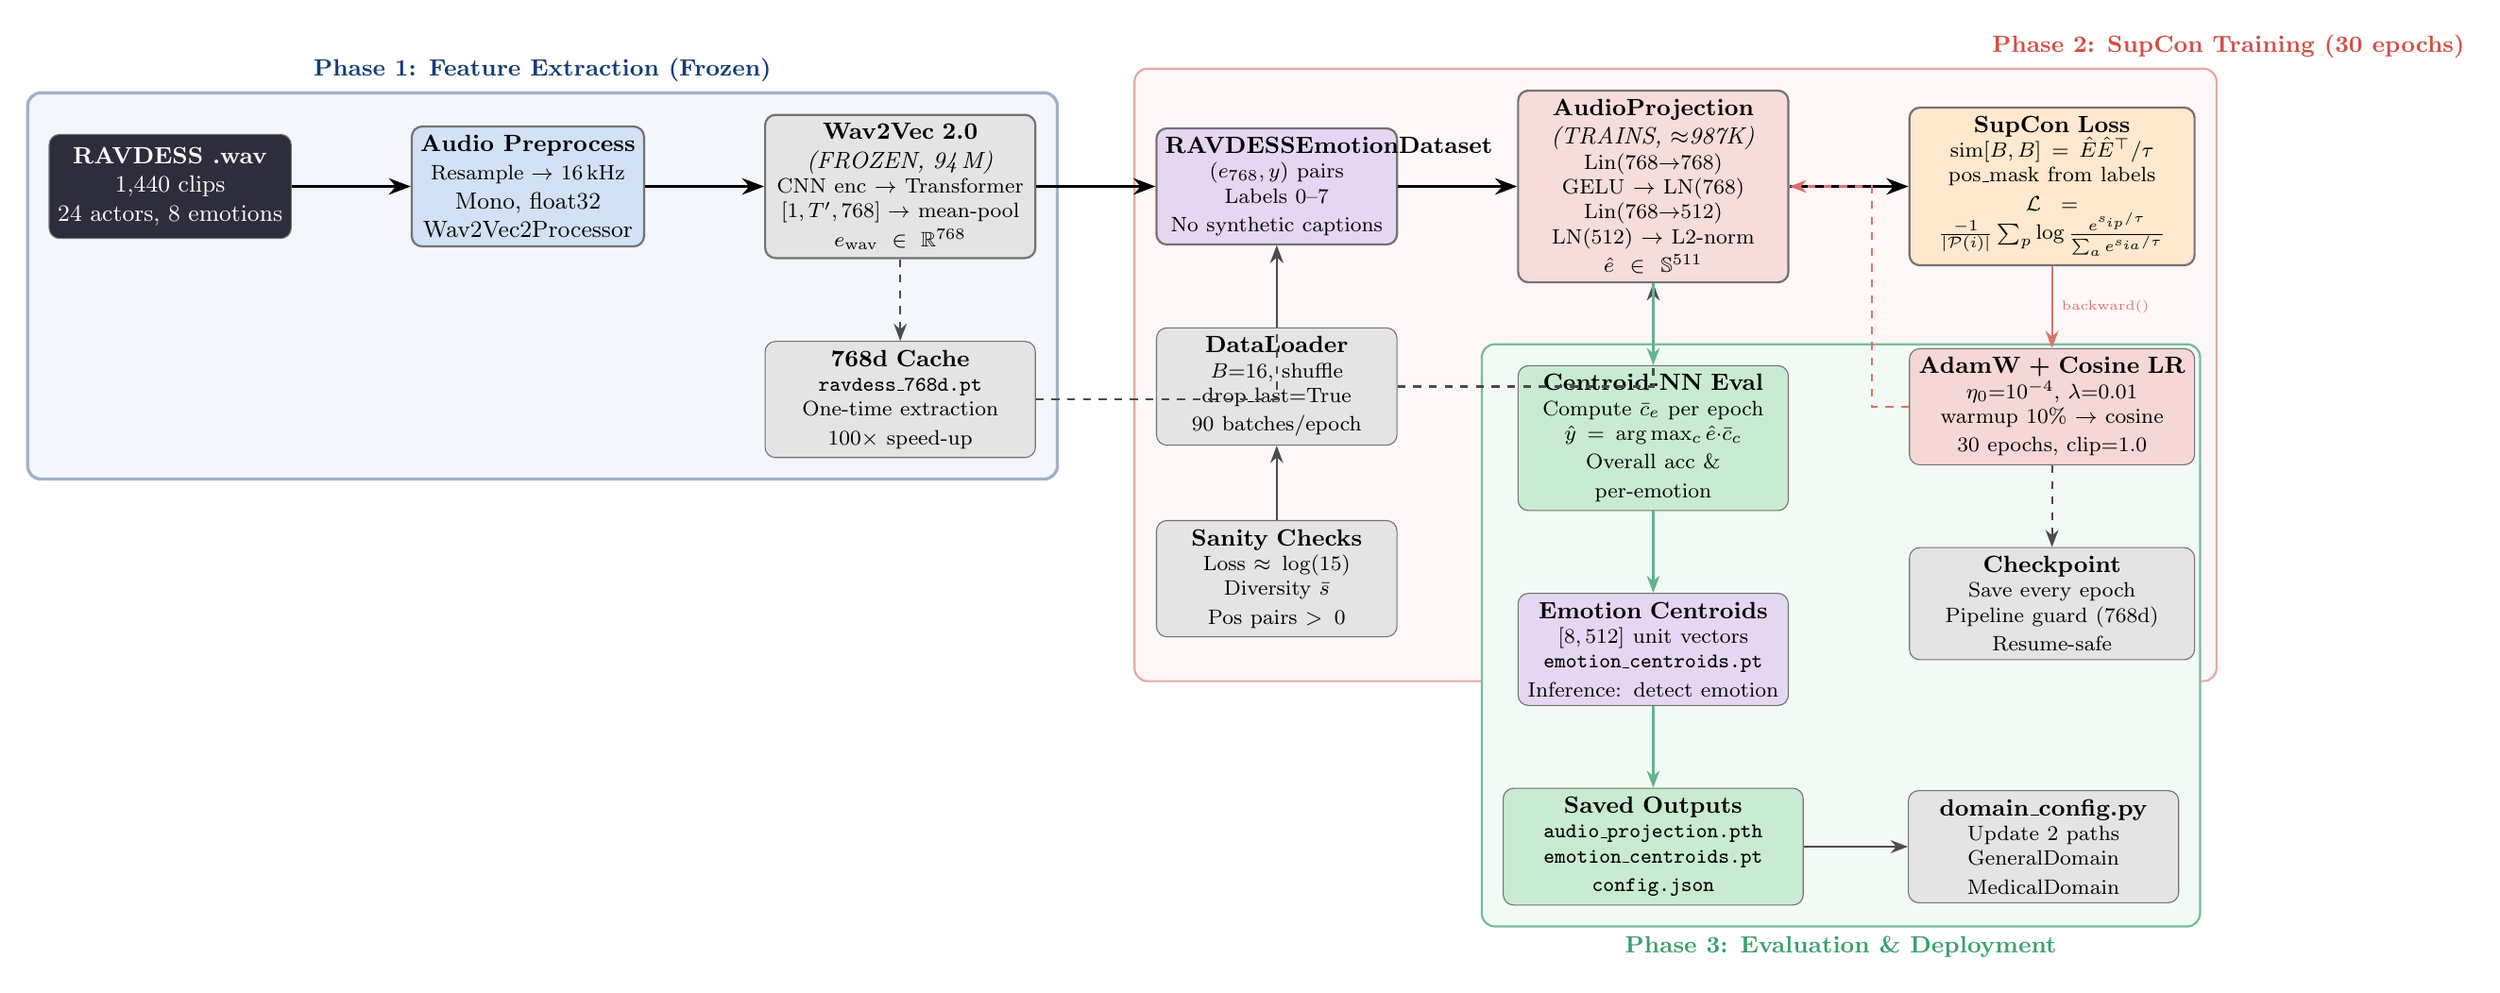
\begin{tikzpicture}[node distance=0.95cm and 1.3cm]

  %% ── ROW 0: INPUT ───────────────────────────────────────────
  \node[inputbox] (wavInput) {
    \textbf{RAVDESS .wav}\\
    $1{,}440$ clips\\
    24 actors, 8 emotions
  };

  %% ── ROW 1: PREPROCESSING ────────────────────────────────────
  \node[procbox, right=1.6cm of wavInput] (preproc) {
    \textbf{Audio Preprocess}\\
    \footnotesize
    Resample $\to$ 16\,kHz\\
    Mono, float32\\
    Wav2Vec2Processor
  };

  %% ── ROW 2: WAV2VEC ──────────────────────────────────────────
  \node[procbox, right=1.6cm of preproc, fill=BoxGray,
        minimum height=1.6cm, text width=3.4cm] (w2v) {
    \textbf{Wav2Vec 2.0}\\
    \textit{(FROZEN, 94\,M)}\\
    \footnotesize
    CNN enc $\to$ Transformer\\
    $[1,T',768] \to$ mean-pool\\
    $e_{\text{wav}} \in \mathbb{R}^{768}$
  };

  %% ── ROW 2: CACHE ───────────────────────────────────────────
  \node[infbox, below=1.1cm of w2v, text width=3.4cm] (cache) {
    \textbf{768d Cache}\\
    \footnotesize
    \texttt{ravdess\_768d.pt}\\
    One-time extraction\\
    $100\times$ speed-up
  };

  %% ── ROW 3: DATASET ──────────────────────────────────────────
  \node[procbox, right=1.6cm of w2v, fill=BoxPurple, text width=3.0cm] (dataset) {
    \textbf{RAVDESSEmotionDataset}\\
    \footnotesize
    $(e_{768}, y) $ pairs\\
    Labels 0–7\\
    No synthetic captions
  };

  %% ── ROW 3b: DATALOADER ──────────────────────────────────────
  \node[infbox, below=1.1cm of dataset, text width=3.0cm] (loader) {
    \textbf{DataLoader}\\
    \footnotesize
    $B{=}16$, shuffle\\
    drop\_last=True\\
    90 batches/epoch
  };

  %% ── ROW 4: AUDIOPROJ ────────────────────────────────────────
  \node[procbox, right=1.6cm of dataset, fill=CoralRed!20,
        minimum height=2.2cm, text width=3.4cm] (audioproj) {
    \textbf{AudioProjection}\\
    \textit{(TRAINS, $\approx$987K)}\\
    \footnotesize
    $\text{Lin}(768{\to}768)$\\
    GELU $\to$ LN(768)\\
    $\text{Lin}(768{\to}512)$\\
    LN(512) $\to$ L2-norm\\
    $\hat{e} \in \mathbb{S}^{511}$
  };

  %% ── ROW 5: SUPCON ───────────────────────────────────────────
  \node[lossbox, right=1.6cm of audioproj, text width=3.6cm] (supcon) {
    \textbf{SupCon Loss}\\
    \footnotesize
    sim$[B,B] = \hat{E}\hat{E}^\top/\tau$\\
    pos\_mask from labels\\
    $\mathcal{L} = \frac{-1}{|\mathcal{P}(i)|}\sum_p \log\frac{e^{s_{ip}/\tau}}{\sum_a e^{s_{ia}/\tau}}$
  };

  %% ── ADAMW ───────────────────────────────────────────────────
  \node[trainbox, below=1.1cm of supcon, text width=3.6cm] (adamw) {
    \textbf{AdamW + Cosine LR}\\
    \footnotesize
    $\eta_0{=}10^{-4}$, $\lambda{=}0.01$\\
    warmup 10\% $\to$ cosine\\
    30 epochs, clip=1.0
  };

  %% ── CHECKPOINT ──────────────────────────────────────────────
  \node[infbox, below=1.1cm of adamw, text width=3.6cm] (ckpt) {
    \textbf{Checkpoint}\\
    \footnotesize
    Save every epoch\\
    Pipeline guard (768d)\\
    Resume-safe
  };

  %% ── EVAL ────────────────────────────────────────────────────
  \node[outbox, below=1.1cm of audioproj, text width=3.4cm] (eval) {
    \textbf{Centroid-NN Eval}\\
    \footnotesize
    Compute $\bar{c}_e$ per epoch\\
    $\hat{y}=\arg\max_c \hat{e}{\cdot}\bar{c}_c$\\
    Overall acc \& per-emotion
  };

  %% ── CENTROIDS ───────────────────────────────────────────────
  \node[centbox, below=1.1cm of eval, text width=3.4cm] (centroids) {
    \textbf{Emotion Centroids}\\
    \footnotesize
    $[8,512]$ unit vectors\\
    \texttt{emotion\_centroids.pt}\\
    Inference: detect emotion
  };

  %% ── OUTPUTS ─────────────────────────────────────────────────
  \node[outbox, below=1.1cm of centroids, text width=3.8cm] (outputs) {
    \textbf{Saved Outputs}\\
    \footnotesize
    \texttt{audio\_projection.pth}\\
    \texttt{emotion\_centroids.pt}\\
    \texttt{config.json}
  };

  %% ── domain_config ───────────────────────────────────────────
  \node[infbox, right=1.4cm of outputs, text width=3.4cm] (domcfg) {
    \textbf{domain\_config.py}\\
    \footnotesize
    Update 2 paths\\
    GeneralDomain\\
    MedicalDomain
  };

  %% ── SANITY ──────────────────────────────────────────────────
  \node[infbox, below=1.0cm of loader, text width=3.0cm] (sanity) {
    \textbf{Sanity Checks}\\
    \footnotesize
    Loss $\approx\log(15)$\\
    Diversity $\bar{s}$\\
    Pos pairs $> 0$
  };

  %% ── ARROWS ──────────────────────────────────────────────────

  % Input chain
  \draw[thickarrow] (wavInput.east) -- (preproc.west);
  \draw[thickarrow] (preproc.east) -- (w2v.west);
  \draw[thickarrow] (w2v.east) -- (dataset.west);
  \draw[thickarrow] (dataset.east) -- (audioproj.west);
  \draw[thickarrow] (audioproj.east) -- (supcon.west);

  % Cache branch
  \draw[arrow, dashed] (w2v.south) -- (cache.north);
  \draw[arrow, dashed] (cache.east) -| ($(dataset.south)+(0,-0.3)$) -- (dataset.south);

  % DataLoader → AudioProj
  \draw[arrow] (loader.north) -- (dataset.south);
  \draw[arrow, dashed] (loader.east) -| ($(audioproj.south)+(0,-0.35)$) -- (audioproj.south);
  \draw[arrow] (sanity.north) -- (loader.south);

  % Loss → training
  \draw[redarrow] (supcon.south) -- node[right,font=\tiny]{backward()} (adamw.north);
  \draw[redarrow, dashed] (adamw.west) -| ++(-0.5,0) |- (audioproj.east);

  % Eval chain
  \draw[greenarrow] (audioproj.south) -- (eval.north);
  \draw[greenarrow] (eval.south) -- (centroids.north);
  \draw[greenarrow] (centroids.south) -- (outputs.north);
  \draw[arrow] (outputs.east) -- (domcfg.west);

  % Checkpoint
  \draw[arrow, dashed] (adamw.south) -- (ckpt.north);

  %% ── BACKGROUND CONTAINERS ────────────────────────────────────
  \begin{pgfonlayer}{background}
    % Extraction phase
    \node[rectangle,draw=NavyBlue!40,fill=DarkContainer!20,rounded corners=5pt,
          very thick,
          fit=(wavInput)(preproc)(w2v)(cache),
          inner sep=8pt,
          label={[font=\small\bfseries,color=NavyBlue]above:%
                 Phase 1: Feature Extraction (Frozen)}] {};

    % Training phase
    \node[rectangle,draw=CoralRed!50,fill=BoxRed!20,rounded corners=5pt,thick,
          fit=(dataset)(loader)(audioproj)(supcon)(adamw)(ckpt)(sanity),
          inner sep=8pt,
          label={[font=\small\bfseries,color=CoralRed]above right:%
                 Phase 2: SupCon Training (30 epochs)}] {};

    % Output phase
    \node[rectangle,draw=MintGreen!70,fill=BoxGreen!25,rounded corners=5pt,thick,
          fit=(eval)(centroids)(outputs)(domcfg),
          inner sep=8pt,
          label={[font=\small\bfseries,color=MintGreen]below:%
                 Phase 3: Evaluation \& Deployment}] {};
  \end{pgfonlayer}

\end{tikzpicture}
}%
\caption{Pipeline~C complete data-flow diagram.
\textcolor{NavyBlue}{\textbf{Blue}} = frozen feature extraction.
\textcolor{CoralRed}{\textbf{Red}} = SupCon training and optimisation.
\textcolor{MintGreen}{\textbf{Green}} = evaluation and deployment outputs.
Dashed arrows = optional/resume paths and gradient flow.}
\label{fig:pipeline}
\end{figure}

% ============================================================
\section{RAVDESS Dataset and Filename Parsing}
% ============================================================

\subsection{Dataset Properties}

\begin{definition}[RAVDESS Dataset]
The Ryerson Audio-Visual Database of Emotional Speech and Song (RAVDESS) is a
validated multimodal dataset comprising 1,440 audio speech clips performed by
24 professional actors (12 female, 12 male), each expressing 8 emotion categories
at normal and strong intensities.  Pipeline~C uses only the audio-speech subset
(modality code~03, vocal channel code~01).
\end{definition}

\subsection{Filename Encoding}

RAVDESS filenames encode all metadata using a standardised 7-field hyphen-delimited format:

\begin{center}
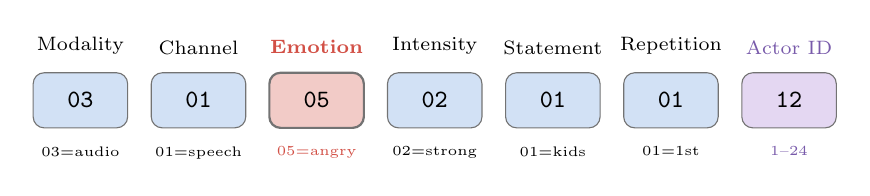
\begin{tikzpicture}[every node/.style={font=\small}]
  \node[basebox,fill=BoxBlue,minimum width=1.2cm,minimum height=0.7cm] (p1) at (0,0) {\texttt{03}};
  \node[basebox,fill=BoxBlue,minimum width=1.2cm,minimum height=0.7cm] (p2) at (1.5,0) {\texttt{01}};
  \node[basebox,fill=CoralRed!30,minimum width=1.2cm,minimum height=0.7cm,thick] (p3) at (3.0,0) {\texttt{05}};
  \node[basebox,fill=BoxBlue,minimum width=1.2cm,minimum height=0.7cm] (p4) at (4.5,0) {\texttt{02}};
  \node[basebox,fill=BoxBlue,minimum width=1.2cm,minimum height=0.7cm] (p5) at (6.0,0) {\texttt{01}};
  \node[basebox,fill=BoxBlue,minimum width=1.2cm,minimum height=0.7cm] (p6) at (7.5,0) {\texttt{01}};
  \node[basebox,fill=BoxPurple,minimum width=1.2cm,minimum height=0.7cm] (p7) at (9.0,0) {\texttt{12}};
  \node[above=3pt of p1,font=\scriptsize] {Modality};
  \node[above=3pt of p2,font=\scriptsize] {Channel};
  \node[above=3pt of p3,font=\scriptsize,color=CoralRed] {\textbf{Emotion}};
  \node[above=3pt of p4,font=\scriptsize] {Intensity};
  \node[above=3pt of p5,font=\scriptsize] {Statement};
  \node[above=3pt of p6,font=\scriptsize] {Repetition};
  \node[above=3pt of p7,font=\scriptsize,color=Lavender] {Actor~ID};
  \node[below=3pt of p1,font=\tiny] {03=audio};
  \node[below=3pt of p2,font=\tiny] {01=speech};
  \node[below=3pt of p3,font=\tiny,color=CoralRed] {05=angry};
  \node[below=3pt of p4,font=\tiny] {02=strong};
  \node[below=3pt of p5,font=\tiny] {01=kids};
  \node[below=3pt of p6,font=\tiny] {01=1st};
  \node[below=3pt of p7,font=\tiny,color=Lavender] {1--24};
\end{tikzpicture}
\end{center}

\begin{algorithm}[H]
\caption{RAVDESS Filename Parser}
\label{alg:parser}
\begin{algorithmic}[1]
\INPUT{Filename string, e.g.\ \texttt{03-01-05-01-02-01-12.wav}}
\OUTPUT{\{emotion, actor\_id, intensity\} or \texttt{None}}
\State name $\gets$ strip extension; parts $\gets$ name.split(\texttt{'-'})
\If{$|\text{parts}| \neq 7$} \Return \texttt{None} \EndIf
\State modality $\gets$ int(parts[0]); channel $\gets$ int(parts[1])
\State emotion\_id $\gets$ int(parts[2]); intensity $\gets$ int(parts[3])
\State actor\_id $\gets$ int(parts[6])
\If{modality $\neq 3$ \textbf{or} channel $\neq 1$} \Return \texttt{None} \EndIf
\Comment{audio-speech only}
\If{emotion\_id $\notin \{1,\ldots,8\}$} \Return \texttt{None} \EndIf
\State \Return \{EMOTION\_MAP[emotion\_id], actor\_id, `strong' if intensity$=2$ else `normal'\}
\end{algorithmic}
\end{algorithm}

\begin{center}
\renewcommand{\arraystretch}{1.1}
\begin{tabular}{@{}cccc@{}}
\toprule
\textbf{RAVDESS Code} & \textbf{Emotion} & \textbf{Integer Label} & \textbf{Approx.\ clips} \\
\midrule
01 & neutral   & 0 & 180 \\
02 & calm      & 1 & 180 \\
03 & happy     & 2 & 180 \\
04 & sad       & 3 & 180 \\
05 & angry     & 4 & 180 \\
06 & fearful   & 5 & 180 \\
07 & disgust   & 6 & 180 \\
08 & surprised & 7 & 180 \\
\bottomrule
\end{tabular}
\end{center}

\begin{tcolorbox}[layman]
RAVDESS filenames are like barcodes --- each dash-separated number carries specific
information.  The parser reads the third number (emotion code) to label each clip.
We keep only audio-speech files (modality 03, channel 01) and discard song files.
\end{tcolorbox}

% ============================================================
\section{Wav2Vec 2.0 Encoder}
% ============================================================

\subsection{Architecture}

Wav2Vec 2.0 (Baevski et al., NeurIPS 2020) learns speech representations by solving
a contrastive task on masked frames of raw audio waveform.

\begin{figure}[H]
\centering
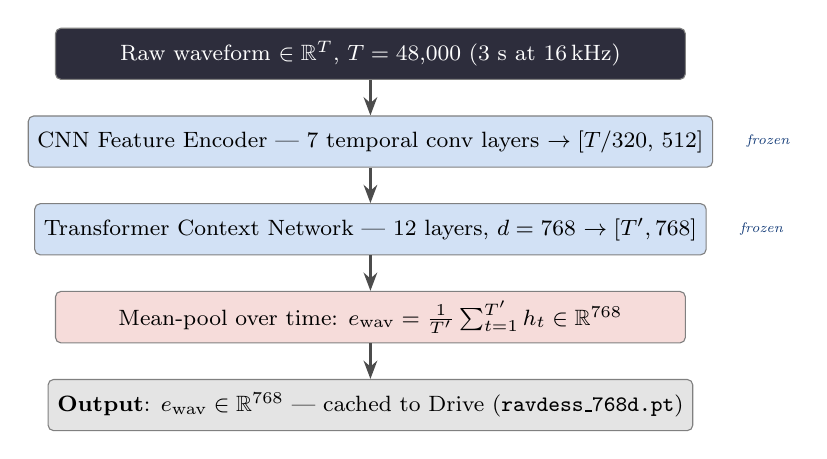
\begin{tikzpicture}[node distance=0.45cm,
  stk/.style={rectangle,rounded corners=2pt,draw=black!50,fill=BoxBlue,
    align=center,font=\footnotesize,minimum width=8cm,minimum height=0.65cm}]
  \node[stk,fill=BoxDark,text=white] (inp) {Raw waveform $\in\mathbb{R}^T$, $T=48{,}000$ (3 s at 16\,kHz)};
  \node[stk,below=of inp] (cnn) {CNN Feature Encoder --- 7 temporal conv layers $\to [T/320,\,512]$};
  \node[stk,below=of cnn] (tf) {Transformer Context Network --- 12 layers, $d=768$ $\to [T',768]$};
  \node[stk,below=of tf,fill=CoralRed!20] (pool) {Mean-pool over time: $e_{\text{wav}} = \tfrac{1}{T'}\sum_{t=1}^{T'} h_t \in\mathbb{R}^{768}$};
  \node[stk,below=of pool,fill=BoxGray] (out) {\textbf{Output}: $e_{\text{wav}} \in \mathbb{R}^{768}$ --- cached to Drive (\texttt{ravdess\_768d.pt})};
  \foreach \a/\b in {inp/cnn,cnn/tf,tf/pool,pool/out}
    \draw[arrow] (\a)--(\b);
  \node[right=0.3cm of cnn,font=\tiny\itshape,color=NavyBlue] {frozen};
  \node[right=0.3cm of tf,font=\tiny\itshape,color=NavyBlue] {frozen};
\end{tikzpicture}
\caption{Wav2Vec 2.0 processing pipeline.  All layers are frozen (zero trainable
parameters during Pipeline~C training).}
\end{figure}

\begin{definition}[Mean-Pool Audio Embedding]
Let $H = [h_1,\ldots,h_{T'}] \in \mathbb{R}^{T'\times 768}$ be the Transformer's
last-layer hidden states.  The mean-pooled sentence embedding is:
\[
  e_{\text{wav}} = \frac{1}{T'}\sum_{t=1}^{T'} h_t \;\in\; \mathbb{R}^{768}
\]
For a 3-second RAVDESS clip: $T\approx48{,}000$, $T'\approx 150$ frames.
\end{definition}

\begin{theorem}[Transfer Learning Efficiency]
\label{thm:transfer}
Freezing Wav2Vec 2.0 (94\,M parameters pre-trained on 960\,h LibriSpeech)
simultaneously achieves:
\begin{enumerate}[nosep]
  \item \textbf{VRAM reduction}: $\approx$360\,MB freed from the training graph.
  \item \textbf{No catastrophic forgetting}: 1,440 clips cannot responsibly update 94\,M parameters.
  \item \textbf{Training speed}: backpropagation skips 94\,M frozen parameters, $\approx$10$\times$ faster per batch.
\end{enumerate}
\end{theorem}

\textbf{Lemma (Caching Speed-up).}
\label{lem:cache}
Each Wav2Vec forward pass on a 3-second clip takes $\approx 0.3$\,s on GPU.
Without caching across 30 training epochs:
\[
  T_{\text{no-cache}} = 1{,}440 \times 30 \times 0.3\,\text{s}
  = 12{,}960\,\text{s} \approx 3.6\,\text{hours}
\]
With one-time caching (120\,s), each epoch reads from CPU memory ($\approx 0.3$\,s total):
\[
  T_{\text{cached}} = 120 + 30 \times 0.3 = 129\,\text{s} \approx 2\,\text{min}
  \qquad \Rightarrow\quad \text{Speed-up} \approx \frac{12{,}960}{129} \approx \mathbf{100\times}
\]

\begin{algorithm}[H]
\caption{Extract and Cache RAVDESS Embeddings at 768d}
\label{alg:cache}
\begin{algorithmic}[1]
\INPUT{RAVDESS\_DIR, CACHE\_768\_FILE}
\OUTPUT{dict: filename $\to$ \{embedding$\in\mathbb{R}^{768}$, emotion, actor\_id, intensity\}}
\If{CACHE\_768\_FILE exists on Drive}
  \State cache $\gets$ \texttt{torch.load}(CACHE\_768\_FILE)
  \State \textbf{assert} cache dim $= 768$ \Comment{dimension guard}
  \State \Return cache \Comment{resume-safe shortcut}
\EndIf
\State encoder $\gets$ Wav2VecEncoder().to(device)
\For{each Actor\_XX directory (24 actors)}
  \For{each \texttt{.wav} file}
    \State meta $\gets$ \textsc{ParseRavdessFilename}(wav\_file)
    \If{meta is None} \textbf{skip} \EndIf
    \State $e \gets$ encoder.encode\_file(wav\_path).squeeze(0) \Comment{$\in\mathbb{R}^{768}$}
    \State cache[wav\_file] $\gets$ \{embedding: $e$, emotion: meta.emotion, \ldots\}
  \EndFor
\EndFor
\State \texttt{torch.save}(cache, CACHE\_768\_FILE)
\State \textbf{del} encoder; \texttt{torch.cuda.empty\_cache}() \Comment{free 360\,MB VRAM}
\State \Return cache
\end{algorithmic}
\end{algorithm}

\begin{tcolorbox}[layman]
Wav2Vec 2.0 is a specialist listener trained on 960 hours of speech.
We borrow its ears (frozen) and run it once on all 1,440 RAVDESS clips,
saving the 768-number fingerprint for each clip.  During the actual training
loop we never touch Wav2Vec again --- we read the saved fingerprints from
Drive, like reading pre-cooked ingredients rather than cooking from scratch
every day.
\end{tcolorbox}

% ============================================================
\section{AudioProjection Architecture}
% ============================================================

\subsection{The wav2vec\_dim Bug --- Fixed}

The original Month~2 AudioProjection used \texttt{wav2vec\_dim=512} because the
cache was wrongly saved at 512d.  This created a near-identity $512\to512$ map
with essentially no useful projection to learn.

\subsection{Formal Definition}

\begin{definition}[AudioProjection]
Let $x \in \mathbb{R}^{768}$ be the cached Wav2Vec mean-pooled embedding.
AudioProjection defines the map:
\[
  f_\theta : \mathbb{R}^{768} \longrightarrow \mathbb{S}^{511}
\]
\[
  f_\theta(x) = \frac{g_\theta(x)}{\|g_\theta(x)\|_2}, \qquad
  g_\theta(x) = \mathrm{LN}_{512}\!\left(W_2 \cdot \mathrm{GELU}\!\left(\mathrm{LN}_{768}(W_1 x + b_1)\right) + b_2\right)
\]
where $W_1 \in \mathbb{R}^{768\times768}$, $W_2 \in \mathbb{R}^{512\times768}$, and
$\mathrm{LN}$ denotes Layer Normalisation.
\end{definition}

\begin{figure}[H]
\centering
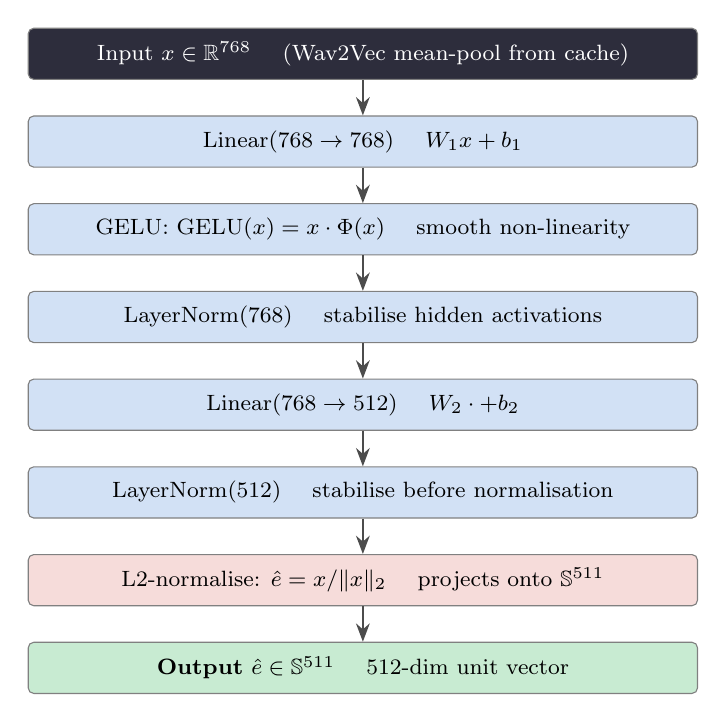
\begin{tikzpicture}[node distance=0.45cm,
  lay/.style={rectangle,rounded corners=2pt,draw=black!50,
    fill=BoxBlue,align=center,font=\footnotesize,
    minimum width=8.5cm,minimum height=0.65cm}]
  \node[lay,fill=BoxDark,text=white] (in) {Input $x\in\mathbb{R}^{768}$ \quad (Wav2Vec mean-pool from cache)};
  \node[lay,below=of in] (l1) {Linear$(768\to768)$ \quad $W_1 x + b_1$};
  \node[lay,below=of l1] (gelu) {GELU: $\text{GELU}(x)=x\cdot\Phi(x)$ \quad smooth non-linearity};
  \node[lay,below=of gelu] (ln1) {LayerNorm(768) \quad stabilise hidden activations};
  \node[lay,below=of ln1] (l2) {Linear$(768\to512)$ \quad $W_2\cdot + b_2$};
  \node[lay,below=of l2] (ln2) {LayerNorm(512) \quad stabilise before normalisation};
  \node[lay,below=of ln2,fill=CoralRed!20] (l2n) {L2-normalise: $\hat{e} = x/\|x\|_2$ \quad projects onto $\mathbb{S}^{511}$};
  \node[lay,below=of l2n,fill=BoxGreen] (out) {\textbf{Output} $\hat{e}\in\mathbb{S}^{511}$ \quad 512-dim unit vector};
  \foreach \a/\b in {in/l1,l1/gelu,gelu/ln1,ln1/l2,l2/ln2,ln2/l2n,l2n/out}
    \draw[arrow] (\a)--(\b);
\end{tikzpicture}
\caption{AudioProjection layer-by-layer architecture.}
\label{fig:audioproj}
\end{figure}

\begin{center}
\renewcommand{\arraystretch}{1.15}
\begin{tabular}{@{}lll@{}}
\toprule
\textbf{Layer} & \textbf{Parameters} & \textbf{Total} \\
\midrule
Linear$(768\to768)$ & $768^2 + 768$ & 590,592 \\
LayerNorm$(768)$ & $2\times768$ & 1,536 \\
Linear$(768\to512)$ & $768\times512+512$ & 393,728 \\
LayerNorm$(512)$ & $2\times512$ & 1,024 \\
\midrule
\textbf{Total trainable} & & $\approx$\textbf{986,880} \\
\bottomrule
\end{tabular}
\end{center}

\begin{lemma}[Unit Sphere Alignment]
\label{lem:alignment}
If $\hat{e}_t = f_T(c)$ (TextProjection) and $\hat{e}_a = f_\theta(x)$
(AudioProjection) both lie on $\mathbb{S}^{511}$, then:
\[
  \cos(\hat{e}_t, \hat{e}_a) = \hat{e}_t \cdot \hat{e}_a \;\in\; [-1,+1]
\]
making cosine similarity equivalent to the inner product --- the standard
metric used in FAISS and the MIVA-KNIGHT retrieval pipeline.
\end{lemma}

\begin{tcolorbox}[layman]
AudioProjection is a small translator with about 987,000 adjustable knobs.
It takes the 768-number Wav2Vec fingerprint and squeezes it into a 512-number
direction on an abstract sphere.  After training, ``angry'' clips point in one
direction and ``calm'' clips point in a very different direction.
The L2-norm ensures all clips have the same length (= 1), so we compare only
directions, never magnitudes.
\end{tcolorbox}

% ============================================================
\section{Supervised Contrastive Loss (SupCon)}
% ============================================================

\subsection{Why SupCon instead of InfoNCE?}

\begin{center}
\renewcommand{\arraystretch}{1.15}
\begin{tabular}{@{}lll@{}}
\toprule
\textbf{Property} & \textbf{InfoNCE} & \textbf{SupCon} \\
\midrule
Requires          & 2 paired modalities      & Emotion labels only \\
Positives/anchor  & Exactly 1                & All same-class clips in batch \\
Works without text? & No                     & Yes \\
Multi-class?      & No natural support       & Designed for $C$ classes \\
Used in           & Pipelines A \& B         & \textbf{Pipeline C} \\
\bottomrule
\end{tabular}
\end{center}

\subsection{Mathematical Formulation}

\begin{definition}[Supervised Contrastive Loss]
For a batch $I=\{1,\ldots,B\}$ with emotion labels $\{y_i\}$, let:
\[
  \mathcal{P}(i) = \{p \in I \setminus \{i\} \mid y_p = y_i\}
  \quad\text{(same-emotion set, excluding self)}
\]
\[
  A(i) = I \setminus \{i\} \quad\text{(denominator set)}
\]
The SupCon loss is:
\begin{equation}\label{eq:supcon}
\boxed{
\mathcal{L}_{\mathrm{SupCon}} =
\frac{1}{B}\sum_{i=1}^{B}
\frac{-1}{|\mathcal{P}(i)|}
\sum_{p\in\mathcal{P}(i)}
\log\frac{\exp(\hat{e}_i\cdot\hat{e}_p/\tau)}
         {\displaystyle\sum_{a\in A(i)}\exp(\hat{e}_i\cdot\hat{e}_a/\tau)}
}
\end{equation}
where $\hat{e}_i = e_i/\|e_i\|_2$ and $\tau=0.07$ is the temperature.
\end{definition}

\begin{algorithm}[H]
\caption{SupCon Loss Computation}
\label{alg:supcon}
\begin{algorithmic}[1]
\INPUT{embeddings $E\in\mathbb{R}^{B\times D}$, labels $y\in\mathbb{Z}^B$, temperature $\tau$}
\OUTPUT{Scalar loss}
\State $E \gets E / \|E\|_2$ \Comment{L2-normalise each row}
\State sim $\gets E E^\top / \tau$ \Comment{similarity matrix $[B,B]$}
\State pos\_mask$[i,j] \gets \mathbf{1}[y_i{=}y_j \wedge i{\neq}j]$ \Comment{positive pair indicator}
\State $\text{sim} \gets \text{sim} - \max(\text{sim},\,\text{dim=1})$ \Comment{log-sum-exp stability}
\State exp\_sim $\gets \exp(\text{sim}) \odot (1-I_B)$ \Comment{exclude self from denominator}
\State log\_prob $\gets \text{sim} - \log(\text{exp\_sim.sum}(\text{dim=1}) + \varepsilon)$ \Comment{$[B,B]$}
\State $n_{\text{pos}} \gets \text{pos\_mask.sum}(\text{dim=1})$ \Comment{positives per anchor}
\State valid $\gets (n_{\text{pos}} > 0)$
\If{valid.sum() $= 0$} \Return $0$ \Comment{no positive pairs in batch} \EndIf
\State per\_anchor $\gets -(\text{pos\_mask}\odot\text{log\_prob}).\text{sum}(\text{dim=1})$
\State \Return mean(per\_anchor[valid] / $n_{\text{pos}}$[valid])
\end{algorithmic}
\end{algorithm}

\begin{theorem}[SupCon Random Baseline]
\label{thm:random}
For a uniformly random model with $B=16$ balanced over $C=8$ classes
($|\mathcal{P}(i)|\approx 1$, 14 negatives per anchor):
\[
  \mathcal{L}_{\mathrm{SupCon}}^{\mathrm{random}} \approx \log(B-1) = \log(15) \approx 2.71
\]
After healthy convergence (30 epochs), the target is $\mathcal{L} < 1.0$.
\end{theorem}

\begin{lemma}[Temperature Effect on Gradient Magnitude]
\[
\left\|\frac{\partial\mathcal{L}}{\partial S_{ij}}\right\| \propto \frac{1}{\tau}
\]
At $\tau=0.07$, gradients are $\approx 14\times$ larger than at $\tau=1.0$,
producing tighter, more discriminative emotion clusters.
\end{lemma}

\begin{lemma}[Positive Pair Existence]
SupCon produces non-zero gradients only when $|\mathcal{P}(i)|>0$ for at least
one anchor.  With \texttt{drop\_last=True} and $B=16$ over 8 balanced classes,
each batch in expectation contains $\lfloor16/8\rfloor=2$ clips per emotion,
guaranteeing at least 1 positive pair per anchor in expectation.
\end{lemma}

\begin{tcolorbox}[layman]
SupCon is a team-building exercise.  Each audio clip looks at all 15 other clips
in its batch.  Same-emotion clips (teammates) are rewarded for pointing in similar
directions; different-emotion clips (opponents) are penalised for being too similar.
Temperature $\tau=0.07$ makes the grader very strict --- only genuinely close
teammates receive a good score.  Unlike InfoNCE, there is no ``other modality''
required: the emotion label alone defines who the teammates are.
\end{tcolorbox}

% ============================================================
\section{AdamW Optimiser and Learning Rate Schedule}
% ============================================================

\subsection{AdamW Update Rule}

\begin{definition}[AdamW]
At step $t$ with gradient $\nabla_t$:
\[
  m_t = \beta_1 m_{t-1}+(1-\beta_1)\nabla_t, \quad
  v_t = \beta_2 v_{t-1}+(1-\beta_2)\nabla_t^2
\]
\[
  \hat{m}_t = m_t/(1-\beta_1^t), \quad \hat{v}_t = v_t/(1-\beta_2^t)
\]
\[
  \theta_{t+1} = \theta_t
  - \eta_t\cdot\frac{\hat{m}_t}{\sqrt{\hat{v}_t}+\varepsilon}
  \;-\; \underbrace{\eta_t\lambda\theta_t}_{\text{weight decay}}
\]
Pipeline~C: $\beta_1{=}0.9$, $\beta_2{=}0.999$, $\varepsilon{=}10^{-8}$,
$\lambda{=}0.01$, $\eta_0{=}10^{-4}$.
\end{definition}

\subsection{Warmup + Cosine Decay Schedule}

\begin{definition}[Warmup + Cosine LR Schedule]
Let $T_{\max} = 90 \times 30 = 2{,}700$ total steps, $t_w = T_{\max}/10 = 270$
warmup steps:
\[
  \eta(t) = \begin{cases}
  \eta_0 \cdot \dfrac{t}{t_w} & t < t_w \quad\text{(linear warmup)}\\[6pt]
  \eta_0 \cdot \dfrac{1}{2}\!\left(1+\cos\dfrac{\pi(t-t_w)}{T_{\max}-t_w}\right) & t\geq t_w \quad\text{(cosine decay)}
  \end{cases}
\]
\end{definition}

\begin{figure}[H]
\centering
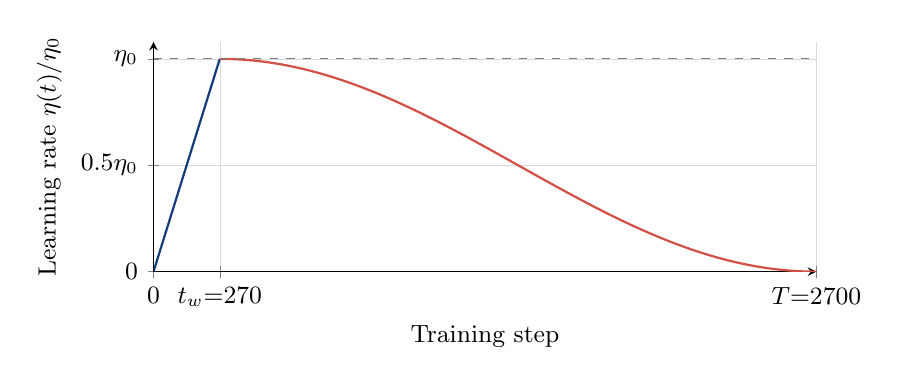
\begin{tikzpicture}
\begin{axis}[
  width=10cm, height=4.5cm,
  xlabel={Training step}, ylabel={Learning rate $\eta(t)/\eta_0$},
  xmin=0, xmax=2700, ymin=0, ymax=1.08,
  xtick={0,270,2700}, xticklabels={0,$t_w{=}270$,$T{=}2700$},
  ytick={0,0.5,1}, yticklabels={0,$0.5\eta_0$,$\eta_0$},
  grid=both, grid style={line width=0.2pt,draw=gray!30},
  axis lines=left, tick label style={font=\small},
  label style={font=\small}
]
\addplot[NavyBlue, thick, domain=0:270, samples=50] {x/270};
\addplot[CoralRed, thick, domain=270:2700, samples=200]
  {0.5*(1+cos(deg((x-270)/(2700-270)*pi))};
\addplot[dashed, gray, domain=0:2700] {1.0};
\end{axis}
\end{tikzpicture}
\caption{Learning rate schedule: linear warmup (0--10\% of steps) followed by
cosine decay (10--100\%).}
\end{figure}

\begin{tcolorbox}[layman]
The learning rate schedule is like accelerating out of a junction:
start slowly (warmup), reach full speed, then gradually brake toward the end.
AdamW remembers the recent direction and variability of gradients and adjusts
each parameter's step size individually --- like a smart cruise control that
adapts to road conditions.
\end{tcolorbox}

% ============================================================
\section{Training Loop}
% ============================================================

\subsection{Single-Epoch Algorithm}

\begin{algorithm}[H]
\caption{Single SupCon Training Epoch}
\label{alg:train_epoch}
\begin{algorithmic}[1]
\INPUT{epoch index, audio\_loader, audio\_proj, optimizer, scheduler}
\OUTPUT{mean epoch SupCon loss}
\State audio\_proj.train()
\State epoch\_losses $\gets [\,]$
\For{each $(E_{\text{batch}}\in\mathbb{R}^{B\times768},\; y_{\text{batch}}\in\mathbb{Z}^B)$ in audio\_loader}
  \State $E_{\text{batch}} \gets E_{\text{batch}}$.to(device) \Comment{$[B,768]$}
  \State $y_{\text{batch}} \gets y_{\text{batch}}$.to(device) \Comment{$[B]$}
  \State $\hat{E} \gets \textsc{AudioProjection}(E_{\text{batch}})$ \Comment{$[B,512]$ on $\mathbb{S}^{511}$}
  \State $\ell \gets \textsc{SupConLoss}(\hat{E}, y_{\text{batch}}, \tau{=}0.07)$
  \State optimizer.zero\_grad(); $\ell$.backward()
  \State \texttt{clip\_grad\_norm\_}(params, $c{=}1.0$)
    \Comment{$\|\nabla\|_2\leq 1.0$}
  \State optimizer.step(); scheduler.step()
  \State epoch\_losses.append($\ell$.item())
\EndFor
\State \Return mean(epoch\_losses)
\end{algorithmic}
\end{algorithm}

\subsection{Gradient Clipping}

\begin{definition}[Gradient Clipping]
The clipped gradient $\tilde{\nabla}_\theta$ is:
\[
  \tilde{\nabla}_\theta = \min\!\left(1,\;\frac{c}{\|\nabla_\theta\|_2}\right)\nabla_\theta,
  \quad c = 1.0
\]
Caps the $\ell_2$-norm of all trainable gradients to $c=1.0$ while
preserving direction.  Prevents large LayerNorm gradient spikes in early
epochs from destabilising training.
\end{definition}

\subsection{Full Training Algorithm}

\begin{algorithm}[H]
\caption{Pipeline C Full Training Loop}
\label{alg:full_train}
\begin{algorithmic}[1]
\INPUT{NUM\_EPOCHS=30, audio\_loader, audio\_proj, optimizer, scheduler}
\OUTPUT{best\_state\_dict (highest centroid-NN accuracy)}
\State start\_epoch, all\_losses, all\_accs $\gets$ \textsc{LoadCheckpoint}()
\State best\_acc $\gets \max$(all\_accs) if all\_accs else $0$
\State best\_state\_dict $\gets$ \texttt{None}
\For{epoch $=$ start\_epoch \textbf{to} NUM\_EPOCHS$-1$}
  \State epoch\_loss $\gets$ \textsc{TrainEpoch}(epoch) \Comment{Alg.~\ref{alg:train_epoch}}
  \State acc, per\_emotion, \_ $\gets$ \textsc{EvaluateEmotionAccuracy}() \Comment{Sec.~\ref{sec:eval}}
  \State all\_losses.append(epoch\_loss); all\_accs.append(acc)
  \If{acc $>$ best\_acc}
    \State best\_acc $\gets$ acc; best\_epoch $\gets$ epoch+1
    \State best\_state\_dict $\gets$ deep copy of audio\_proj.state\_dict()
  \EndIf
  \State \textsc{SaveCheckpoint}(epoch, all\_losses, all\_accs) \Comment{every epoch}
  \State print: epoch, loss, accuracy, $n_{\text{correct}}/8$
\EndFor
\State \Return best\_state\_dict
\end{algorithmic}
\end{algorithm}

\begin{center}
\renewcommand{\arraystretch}{1.1}
\begin{tabular}{@{}llll@{}}
\toprule
\textbf{Epoch} & \textbf{Expected loss} & \textbf{Expected accuracy} & \textbf{Interpretation} \\
\midrule
1 & 2.0--2.6 & 20--35\% & Near random; projection uninitialised \\
5 & 1.4--2.0 & 35--55\% & Broad emotion clusters forming \\
10 & 1.0--1.6 & 50--70\% & High-arousal emotions separating \\
20 & 0.6--1.2 & 65--80\% & Most emotions well separated \\
30 & 0.3--0.9 & 75--90\% & Fine-grained within-class compaction \\
\bottomrule
\end{tabular}
\end{center}

\begin{tcolorbox}[layman]
The training loop runs 30 complete study sessions. Each session covers all
1,440 clips in 90 batches of 16. For each batch: AudioProjection maps clips
to 512-d directions, SupCon measures how poorly same-emotion clips cluster,
and backpropagation nudges the model's 987K parameters to improve clustering.
After every session we save to Drive so a Colab disconnect loses only the
current epoch, not all progress.
\end{tcolorbox}

% ============================================================
\section{Emotion Accuracy Evaluation}
\label{sec:eval}
% ============================================================

\subsection{Centroid Nearest-Neighbour Classifier}

\begin{definition}[Spherical Centroid]
For emotion class $e$ with $N_e$ projected embeddings
$\{\hat{a}_1^{(e)},\ldots,\hat{a}_{N_e}^{(e)}\}$ on $\mathbb{S}^{511}$:
\[
  \bar{c}_e = \frac{\mu_e}{\|\mu_e\|_2},
  \quad \mu_e = \frac{1}{N_e}\sum_{i=1}^{N_e}\hat{a}_i^{(e)} \in\mathbb{R}^{512}
\]
\end{definition}

\begin{definition}[Voronoi Centroid Classifier]
The centroid classifier assigns each embedding $\hat{e}$ to the nearest class:
\[
  \hat{y} = \arg\max_{c\in\{0,\ldots,7\}} \hat{e}\cdot\bar{c}_c
\]
This partitions $\mathbb{S}^{511}$ into 8 Voronoi cells.
\end{definition}

\begin{algorithm}[H]
\caption{Evaluate Emotion Accuracy (Centroid-NN)}
\label{alg:eval}
\begin{algorithmic}[1]
\INPUT{audio\_proj, audio\_loader}
\OUTPUT{overall\_acc, per\_emotion (dict), centroids $[8,512]$}
\State audio\_proj.eval()
\State all\_embs $\gets$ cat$\bigl([$audio\_proj$(E_b)$ for $(E_b,y_b)\in$ loader$]\bigr)$ \Comment{$[N,512]$}
\State all\_labels $\gets$ cat$\bigl([y_b]_{b}\bigr)$ \Comment{$[N]$}
\For{$l = 0$ \textbf{to} $7$}
  \State mask $\gets$ (all\_labels $= l$); $\mu_l\gets$ mean(all\_embs[mask], dim=0)
  \State $\bar{c}_l \gets \mu_l/\|\mu_l\|_2$ \Comment{spherical centroid}
\EndFor
\State centroids $\gets$ stack$(\bar{c}_0,\ldots,\bar{c}_7)$ \Comment{$[8,512]$}
\State sims $\gets$ all\_embs $\cdot$ centroids$^\top$ \Comment{$[N,8]$, cosine sims}
\State predicted $\gets$ argmax(sims, dim=1) \Comment{$[N]$}
\State correct $\gets$ (predicted $=$ all\_labels).float()
\State overall\_acc $\gets$ mean(correct)
\For{$l = 0$ \textbf{to} $7$}
  \State per\_emotion[LABEL\_TO\_EMOTION[$l$]] $\gets$ mean(correct[all\_labels $= l$])
\EndFor
\State audio\_proj.train(); \Return overall\_acc, per\_emotion, centroids
\end{algorithmic}
\end{algorithm}

\begin{lemma}[Best-Epoch Selection]
Let $\mathrm{acc}(e)$ be the centroid-NN accuracy at epoch $e$.
The optimal model is $\theta^* = \theta_{\hat{e}}$ where
$\hat{e} = \arg\max_e \mathrm{acc}(e)$.
This model minimises the expected error of the Voronoi centroid classifier
on the RAVDESS training distribution and is the operationally best checkpoint
for MIVA-KNIGHT emotion inference.
\end{lemma}

\begin{tcolorbox}[layman]
After each training epoch, we compute the ``average fingerprint'' (centroid)
for each emotion, then test every clip: does it land closest to its own
emotion's centroid?  This gives an accuracy score from 0\% (random) to
100\% (perfect), with no additional training required.
The per-emotion breakdown reveals which emotions confuse each other
(e.g., neutral and calm both have low arousal and are often adjacent in the space).
\end{tcolorbox}

% ============================================================
\section{Pre-Training Sanity Checks}
% ============================================================

Three diagnostic checks run before training commits to 30 epochs:

\begin{theorem}[Sanity Check 1 --- Loss at Random Init]
For $B=16$ balanced over $C=8$ emotions ($|\mathcal{P}(i)|\approx1$,
14 negatives):
\[
  \mathcal{L}_{\mathrm{SupCon}}^{\mathrm{random}} \approx \log(15) \approx 2.71
\]
Observed loss outside $[1.0,\,4.0]$ indicates an implementation error.
\end{theorem}

\textbf{Check 2 --- Embedding Diversity:}
\[
  \bar{s}_{\mathrm{pre}} = \frac{2}{n(n-1)}\sum_{i<j}\cos(\hat{e}_i,\hat{e}_j)
\]
Expected pre-training range: $[0.3, 0.7]$.
Post-training target: $\bar{s}_{\mathrm{post}} < \bar{s}_{\mathrm{pre}}$
(SupCon spreads emotion clusters apart).
Failure: $\bar{s}\approx1.0$ (representation collapse).

\textbf{Check 3 --- Positive Pair Count:}
\[
  N_{\mathrm{pos}} = \sum_{c=1}^{C} n_c(n_c-1)
\]
For $B=16$, $C=8$ balanced: $N_{\mathrm{pos}} = 8\times2\times1 = 16$.
If $N_{\mathrm{pos}}=0$, SupCon returns zero gradient.

% ============================================================
\section{Checkpoint System}
% ============================================================

\begin{theorem}[Checkpoint Completeness]
Training can be resumed exactly from epoch $e$ iff the checkpoint contains:
\begin{enumerate}[nosep]
  \item Model weights $\theta_e$ (\texttt{state\_dict})
  \item Optimiser state $\{m_t, v_t\}$ at the final step of epoch $e$
  \item Scheduler step counter $t_e$
\end{enumerate}
Without (2), AdamW's momentum vectors reset to zero, requiring $\approx$1--2
warm-up epochs to rebuild velocity.
\end{theorem}

The checkpoint carries two safety guards:
\[
\text{Guard 1:}\ \texttt{ckpt['pipeline']} \neq \texttt{'C-RAVDESS-standalone'} \Rightarrow \text{start fresh}
\]
\[
\text{Guard 2:}\ \texttt{ckpt['wav2vec\_dim']} \neq 768 \Rightarrow \text{start fresh}
\]

% ============================================================
\section{Emotion Centroids for Inference}
% ============================================================

\begin{algorithm}[H]
\caption{Compute and Save Emotion Centroids}
\label{alg:centroids}
\begin{algorithmic}[1]
\State audio\_proj.eval()
\State emotion\_embs $\gets$ defaultdict(list)
\For{each $(E_b, y_b)$ in audio\_loader}
  \State proj $\gets$ audio\_proj$(E_b$.to(device)).cpu() \Comment{$[B,512]$}
  \For{$(\hat{e}, \ell)$ in zip(proj, $y_b$)}
    \State emotion\_embs[LABEL\_TO\_EMOTION[$\ell$]].append($\hat{e}$)
  \EndFor
\EndFor
\For{emotion $e$ in EMOTIONS\_8}
  \State stack $\gets$ torch.stack(emotion\_embs[$e$]) \Comment{$[N_e,512]$}
  \State $\bar{c}_e \gets$ L2\_norm(mean(stack, dim=0))
\EndFor
\State centroids\_tensor $\gets$ stack($\bar{c}_0,\ldots,\bar{c}_7$) \Comment{$[8,512]$}
\State torch.save(centroids\_tensor, CENTROIDS\_PATH)
\end{algorithmic}
\end{algorithm}

\subsection*{Inference Pipeline Using Centroids}

\begin{figure}[H]
\centering
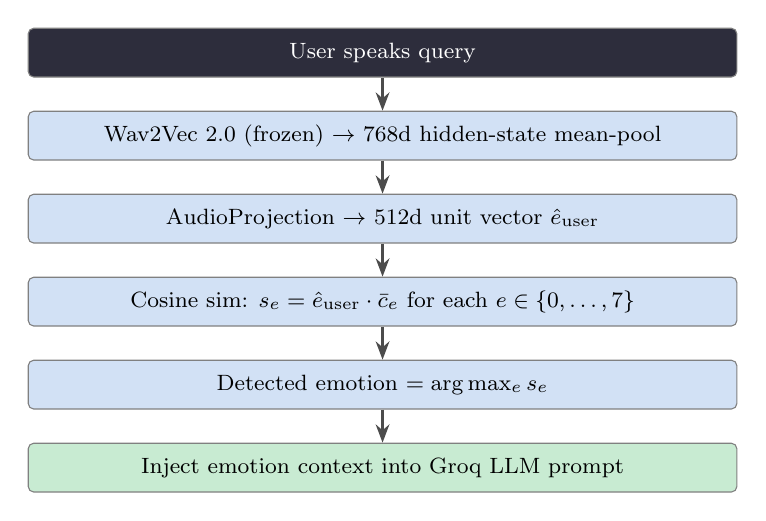
\begin{tikzpicture}[node distance=0.42cm,
  inf/.style={rectangle,rounded corners=2pt,draw=black!50,
    fill=BoxBlue,align=center,font=\footnotesize,minimum width=9cm,minimum height=0.62cm}]
  \node[inf,fill=BoxDark,text=white] (v) {User speaks query};
  \node[inf,below=of v] (wv) {Wav2Vec 2.0 (frozen) $\to$ 768d hidden-state mean-pool};
  \node[inf,below=of wv] (ap) {AudioProjection $\to$ 512d unit vector $\hat{e}_{\text{user}}$};
  \node[inf,below=of ap] (cs) {Cosine sim: $s_e = \hat{e}_{\text{user}}\cdot\bar{c}_e$ for each $e\in\{0,\ldots,7\}$};
  \node[inf,below=of cs] (am) {Detected emotion $= \arg\max_e s_e$};
  \node[inf,below=of am,fill=BoxGreen] (gr) {Inject emotion context into Groq LLM prompt};
  \foreach \a/\b in {v/wv,wv/ap,ap/cs,cs/am,am/gr} \draw[arrow] (\a)--(\b);
\end{tikzpicture}
\caption{MIVA-KNIGHT real-time emotion detection at inference time using
the centroids produced by Pipeline~C.}
\end{figure}

% ============================================================
\section{Outputs and System Integration}
% ============================================================

\subsection{Saved Files}

\begin{center}
\renewcommand{\arraystretch}{1.15}
\begin{tabular}{@{}lllp{3.5cm}@{}}
\toprule
\textbf{File} & \textbf{Format} & \textbf{Shape} & \textbf{Used by} \\
\midrule
\texttt{audio\_projection.pth} & Checkpoint dict & --- & \texttt{pipeline.py}, \texttt{domain\_config.py} \\
\texttt{emotion\_centroids.pt} & Raw tensor & $[8,512]$ & Inference emotion detection \\
\texttt{ravdess\_embeddings\_768d.pt} & Cache dict & $1440\times768$ & Reuse in future runs \\
\texttt{config.json} & JSON & --- & Reproducibility, thesis \\
\texttt{training\_curves.png} & PNG 150\,dpi & --- & Thesis figures \\
\bottomrule
\end{tabular}
\end{center}

\subsection{domain\_config.py Update}

\begin{center}
\renewcommand{\arraystretch}{1.1}
\begin{tabular}{@{}lll@{}}
\toprule
\textbf{Domain} & \textbf{Old path} & \textbf{New path} \\
\midrule
GeneralDomain & \texttt{month2\_rebuilt/audio\_projection.pth} & \texttt{pipelineC/audio\_projection.pth} \\
GeneralDomain & \texttt{month2\_rebuilt/emotion\_centroids.pt} & \texttt{pipelineC/emotion\_centroids.pt} \\
MedicalDomain & (same files) & (same Pipeline C files) \\
\bottomrule
\end{tabular}
\end{center}

% ============================================================
\section{Complete Mathematical Summary}
% ============================================================

\subsection{All Key Equations}

\textbf{Mean-pool embedding (Wav2Vec):}
\[
  e_{\text{wav}} = \frac{1}{T'}\sum_{t=1}^{T'} h_t^{(L)} \;\in\; \mathbb{R}^{768}
\]

\textbf{AudioProjection:}
\[
  f_\theta(x) = \frac{\mathrm{LN}_{512}(W_2\cdot\mathrm{GELU}(\mathrm{LN}_{768}(W_1 x+b_1))+b_2)}
  {\|\mathrm{LN}_{512}(W_2\cdot\mathrm{GELU}(\mathrm{LN}_{768}(W_1 x+b_1))+b_2)\|_2}
  \;\in\; \mathbb{S}^{511}
\]

\textbf{SupCon loss (Equation~\ref{eq:supcon})}

\textbf{AdamW update:}
\[
  \theta_{t+1} = \theta_t - \eta_t\cdot\frac{\hat{m}_t}{\sqrt{\hat{v}_t}+\varepsilon}
  - \eta_t\lambda\theta_t
\]

\textbf{Cosine LR schedule:}
\[
  \eta(t) = \eta_0\cdot\tfrac{1}{2}\!\left(1+\cos\tfrac{\pi(t-t_w)}{T_{\max}-t_w}\right)
  \quad (t\geq t_w)
\]

\textbf{Spherical centroid:}
\[
  \bar{c}_e = \frac{\mu_e}{\|\mu_e\|_2}, \quad
  \mu_e = \frac{1}{N_e}\sum_{i=1}^{N_e}\hat{a}_i^{(e)}
\]

\textbf{Inference emotion detection:}
\[
  \hat{y}_{\text{user}} = \arg\max_{e\in\{0,\ldots,7\}}\;\hat{e}_{\text{user}}\cdot\bar{c}_e
\]

\textbf{Gradient clipping:}
\[
  \tilde{\nabla}_\theta = \min\!\left(1,\frac{1}{\|\nabla_\theta\|_2}\right)\nabla_\theta
\]

\subsection{Notation Reference}

\begin{center}
\renewcommand{\arraystretch}{1.15}
\begin{tabular}{@{}lp{9.5cm}@{}}
\toprule
\textbf{Symbol} & \textbf{Meaning} \\
\midrule
$e_{\text{wav}} \in\mathbb{R}^{768}$ & Wav2Vec mean-pooled audio embedding \\
$\hat{e} \in\mathbb{S}^{511}$ & L2-normalised 512-d audio embedding \\
$W_1,W_2$ & AudioProjection weight matrices \\
$\mathrm{LN}$ & Layer Normalisation \\
$\mathcal{P}(i)$ & Same-emotion batch indices for anchor $i$ \\
$A(i)$ & All-other-sample batch indices for anchor $i$ \\
$\tau$ & SupCon temperature (0.07) \\
$\eta$ & Learning rate \\
$\lambda$ & AdamW weight decay coefficient (0.01) \\
$T_{\max}$ & Total training steps ($90\times30=2700$) \\
$t_w$ & Warmup steps ($T_{\max}/10=270$) \\
$\bar{c}_e$ & Spherical centroid for emotion $e$ \\
$c$ & Gradient clip threshold (1.0) \\
$\bar{s}$ & Mean pairwise cosine similarity (diversity metric) \\
\bottomrule
\end{tabular}
\end{center}

\end{document}
